\IfFileExists{Resources/chapter5/admin-applications.png}{%
Hàng đợi trong Hình~\ref{fig:admin-application-evidence}(a) cung cấp tên, thông tin liên hệ và mô tả hồ sơ xin quyền Host. Admin mở nội dung đầy đủ và tệp giấy tờ trước khi quyết định cấp quyền. Hình~\ref{fig:admin-application-evidence}(b) là hàng đợi minh chứng vị trí và ảnh, hiển thị phòng hoặc tòa nhà cần đối chiếu. Hai hàng đợi phục vụ hai quyết định độc lập: cấp quyền Host và xét duyệt minh chứng không gian.
\begin{figure}[H]
\centering
\begin{minipage}[t]{0.40\linewidth}\centering
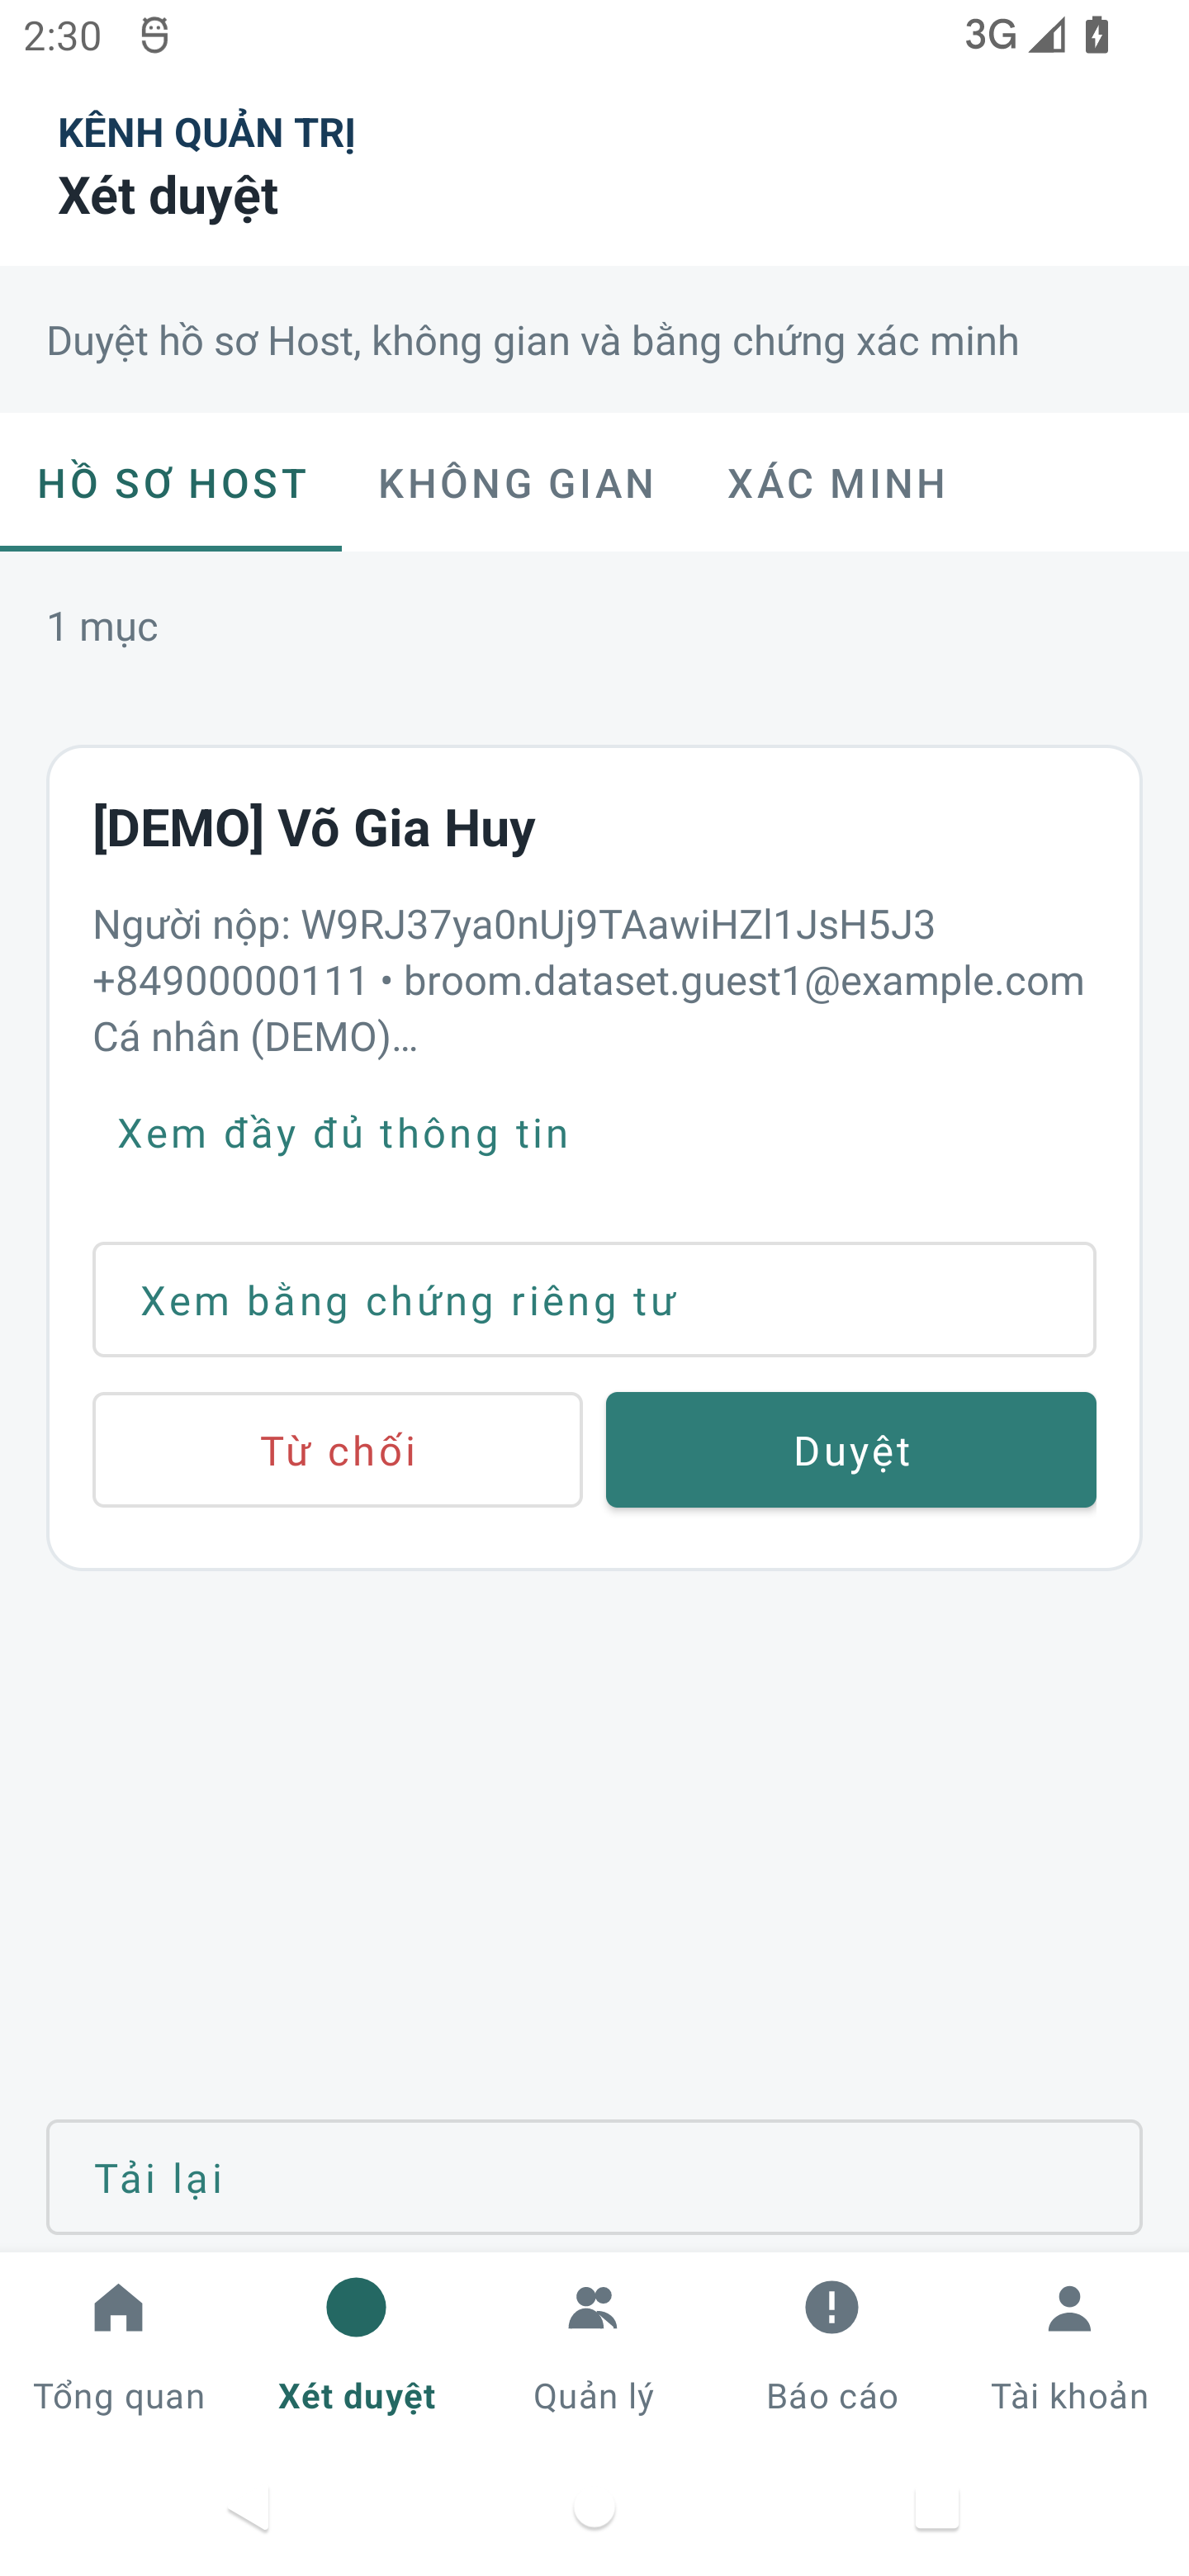
\includegraphics[width=\linewidth]{chapter5/admin-applications.png}\\[-1mm]
{\small (a) Hồ sơ xin quyền Host}
\end{minipage}\hspace{0.05\linewidth}%
\begin{minipage}[t]{0.40\linewidth}\centering
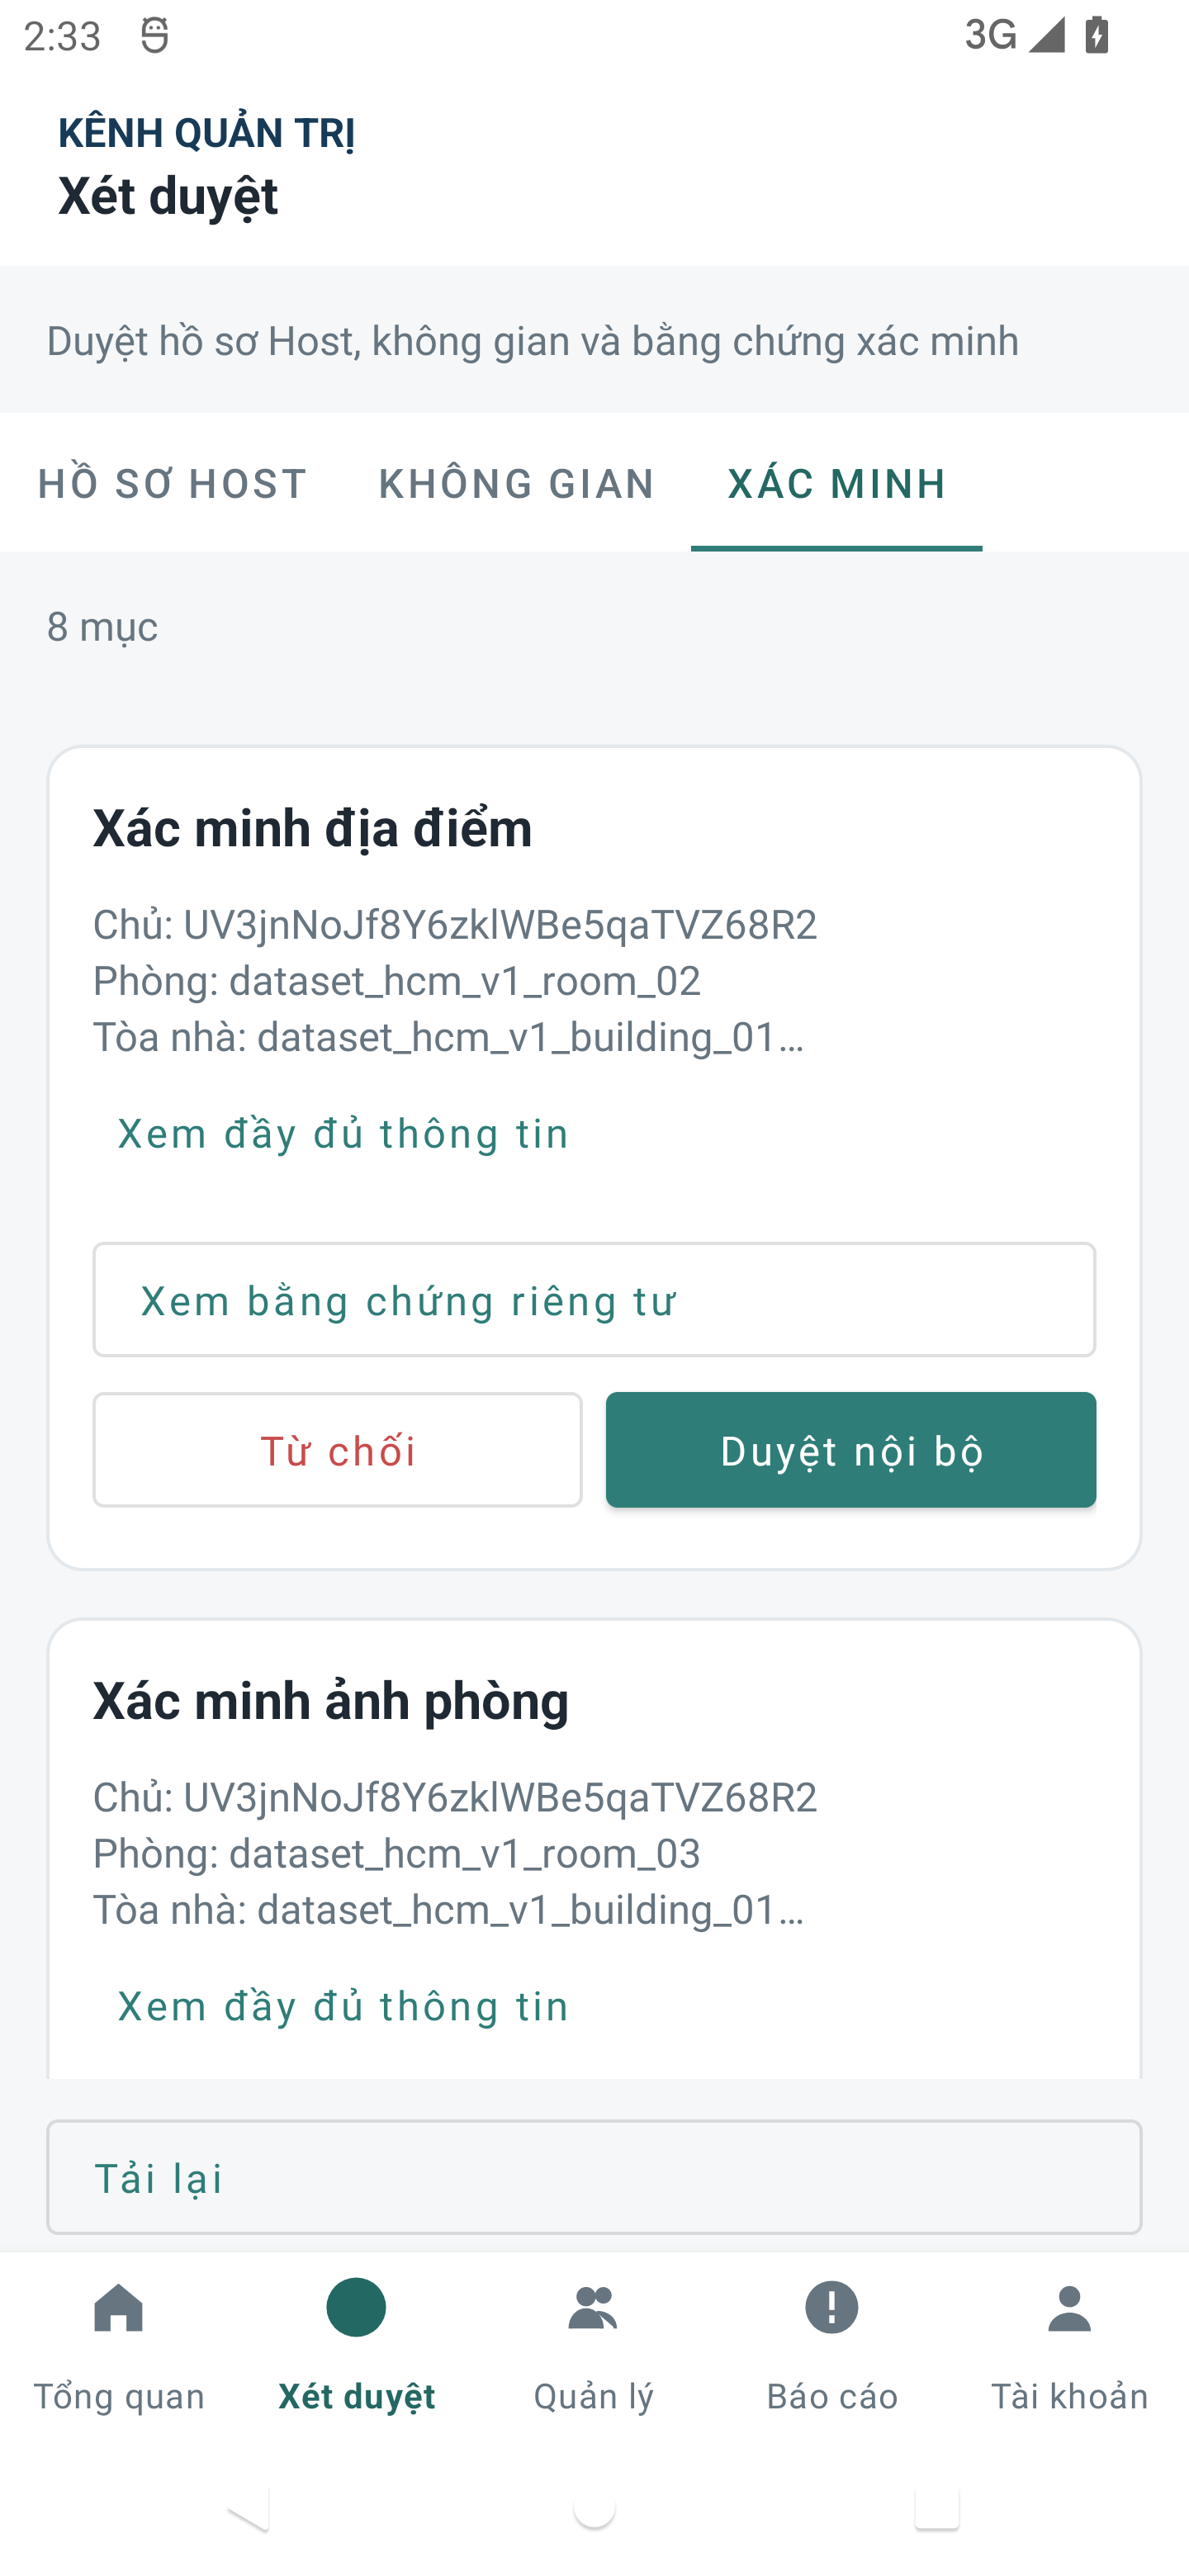
\includegraphics[width=\linewidth]{chapter5/admin-verifications.png}\\[-1mm]
{\small (b) Minh chứng vị trí và ảnh}
\end{minipage}
\caption{Hàng đợi hồ sơ Host và minh chứng không gian}
\label{fig:admin-application-evidence}
\end{figure}}{}

\IfFileExists{Resources/chapter5/admin-hosts.png}{%
Hình~\ref{fig:admin-host-audit}(a) hiển thị tài khoản Host cùng trạng thái hoạt động và thao tác khóa hoặc mở khóa tương ứng. Lý do xử lý được lưu để đối chiếu khi quản lý quyền nhận đặt mới. Nhật ký ở Hình~\ref{fig:admin-host-audit}(b) trình bày hành động, người thực hiện, đối tượng và thay đổi trạng thái theo thời gian. Admin có thể mở nội dung đầy đủ để kiểm tra một quyết định cụ thể; danh sách được giới hạn ở 100 thao tác mới nhất.
\begin{figure}[H]
\centering
\begin{minipage}[t]{0.40\linewidth}\centering
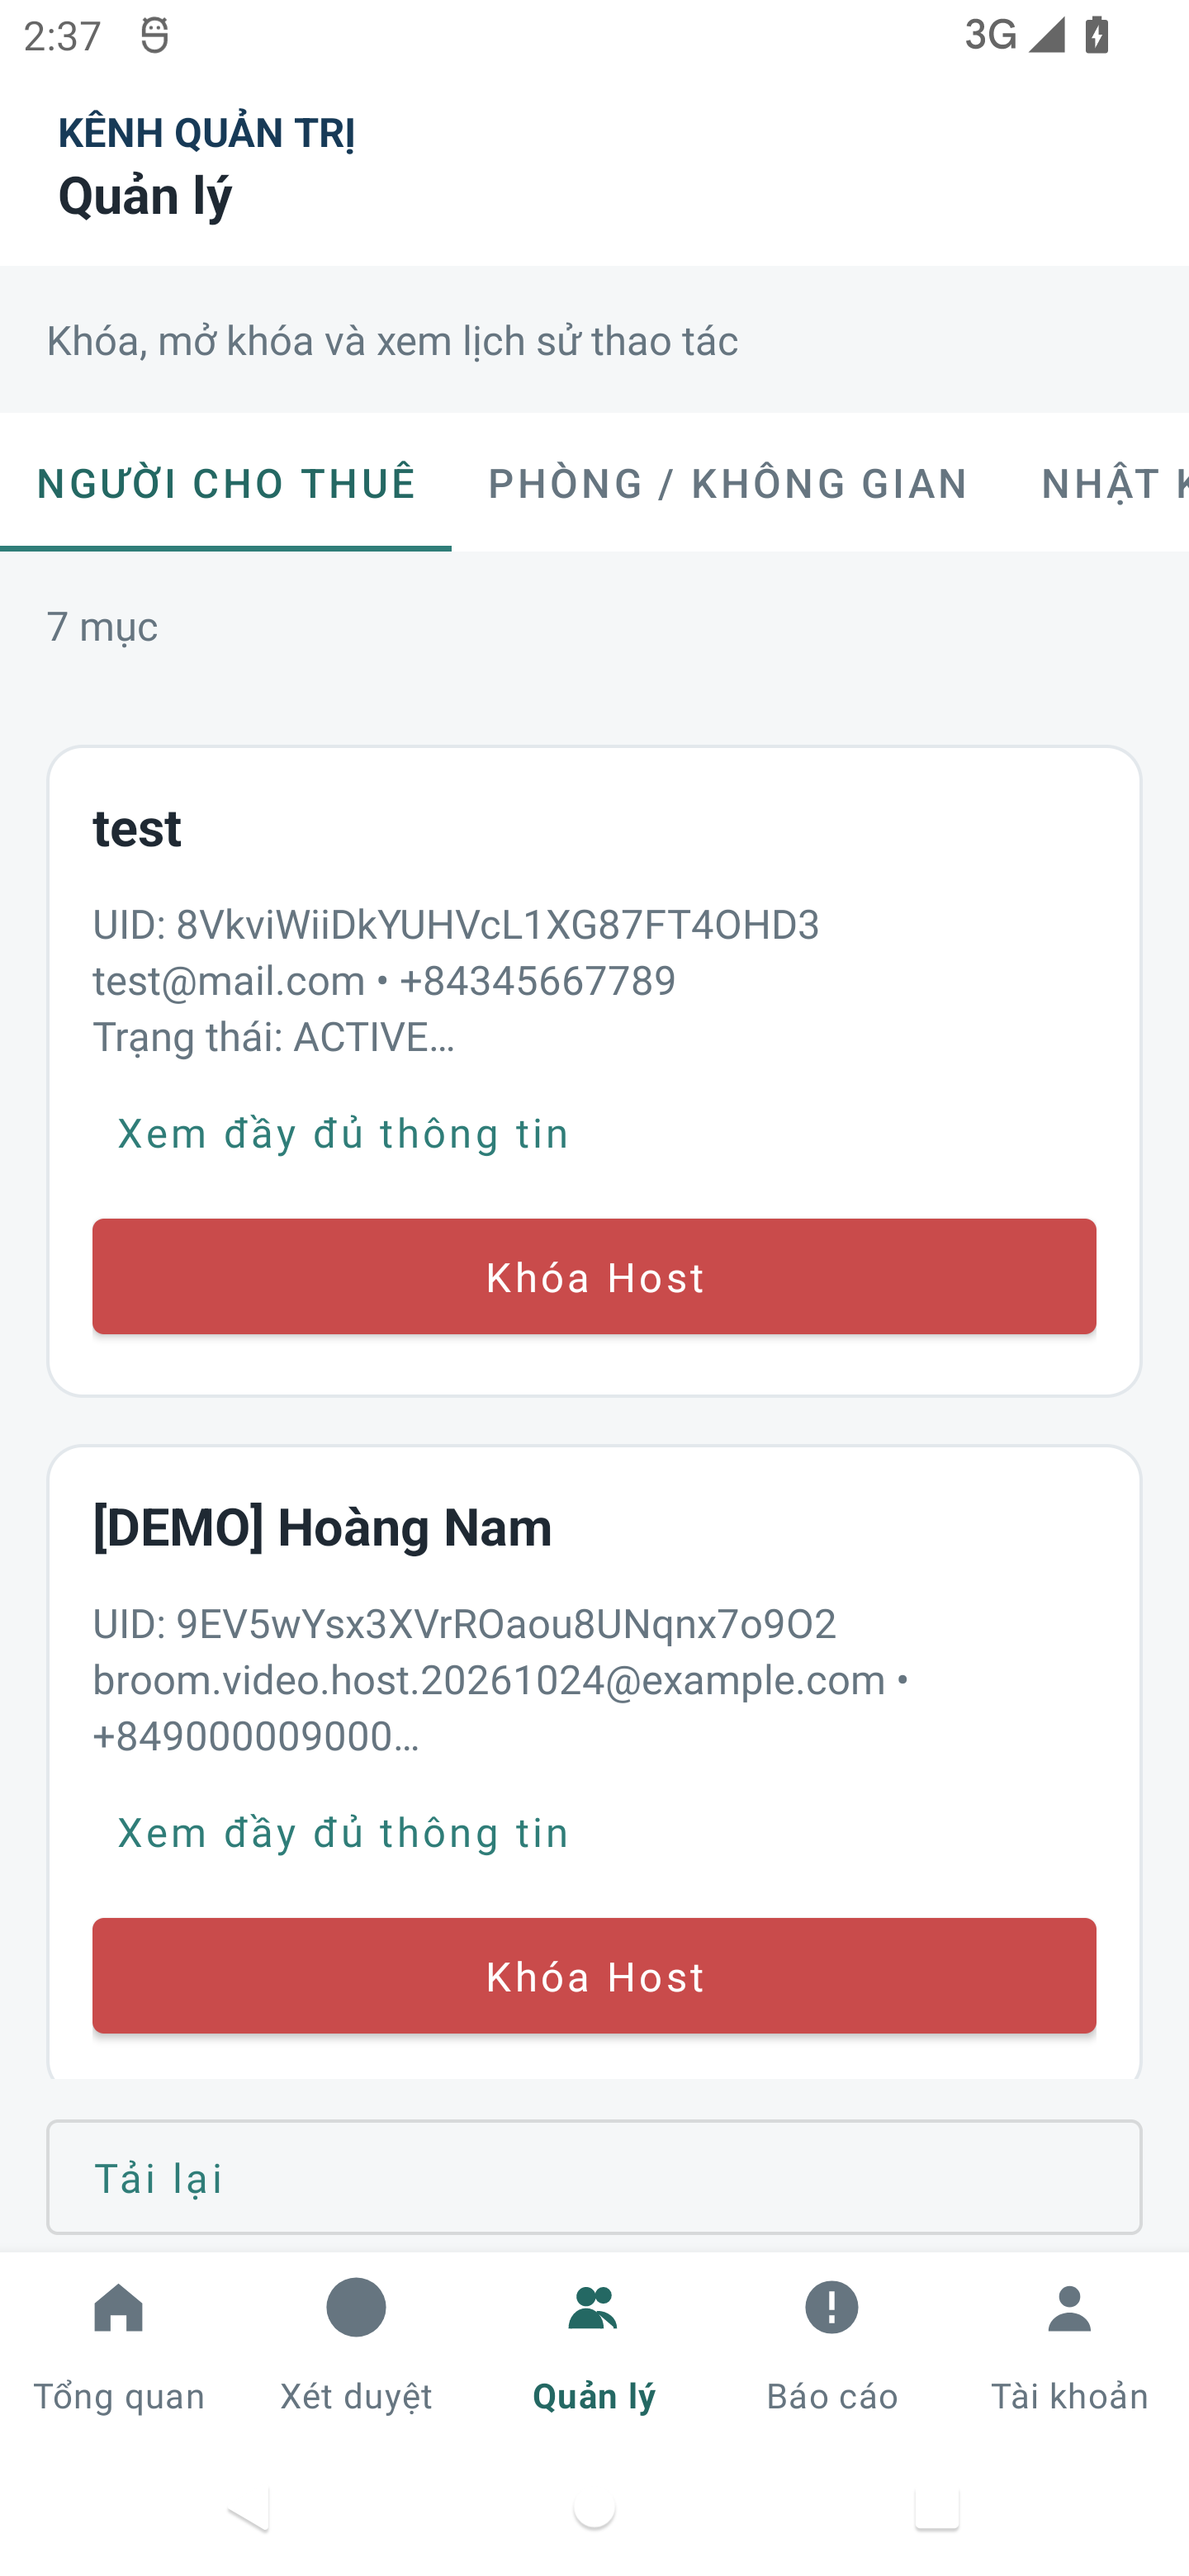
\includegraphics[width=\linewidth]{chapter5/admin-hosts.png}\\[-1mm]
{\small (a) Trạng thái Host}
\end{minipage}\hspace{0.05\linewidth}%
\begin{minipage}[t]{0.40\linewidth}\centering
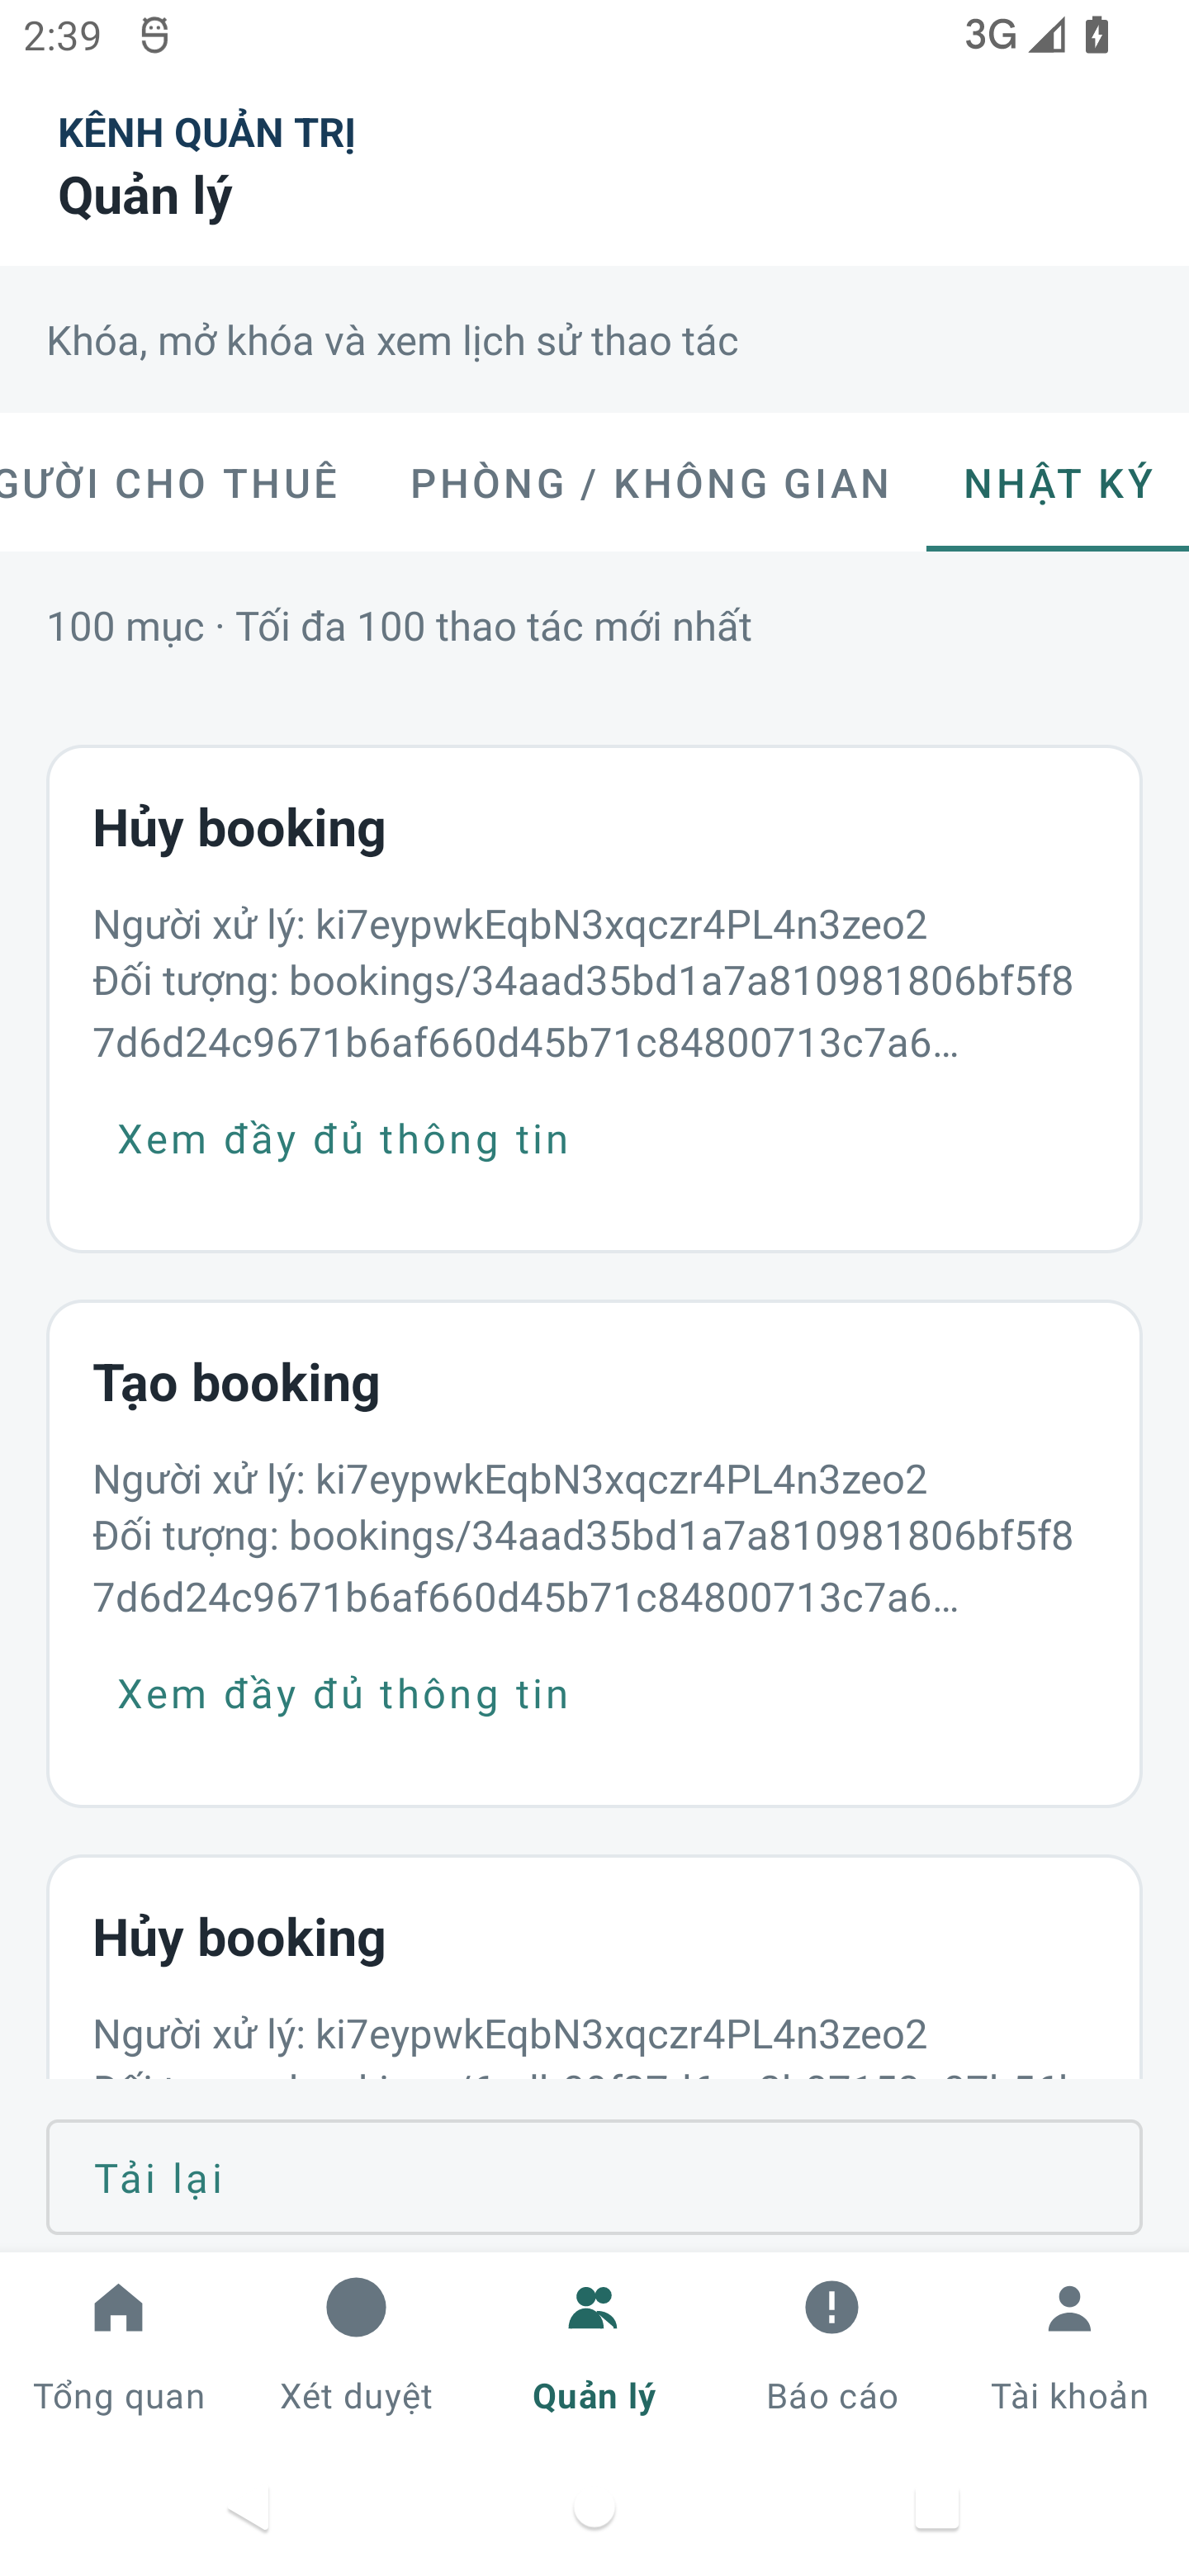
\includegraphics[width=\linewidth]{chapter5/admin-audit.png}\\[-1mm]
{\small (b) Nhật ký nghiệp vụ}
\end{minipage}
\caption{Giao diện quản lý Host và tra cứu nhật ký}
\label{fig:admin-host-audit}
\end{figure}}{}
